% Seccion de Diseno y construccion 

%%\chapter{Integración de componentes}
\label{chapter:diseno}
\section{Diseño y Construcción}

El primer paso ha sido la construcci\'on de la parte física del robot. Para tal fin se procedió a la elección del diseño y ensamblaje de las piezas. En la sección \ref{subsection:componentes} se describe cada uno de los componentes utilizados para armar el robot, y luego, en la secci\'on \ref{subsection:construccion} se explica cómo se integraron esas piezas para obtener un humanoide adaptado a los objetivos de este proyecto.

\label{subsection:componentes}
\subsection{Componentes de hardware}
A continuación se presenta una descripción de todos los elementos utilizados para la construcción del robot humanoide. 

\begin{itemize}
\item Bioloid Premium kit: Es un kit de robótica con piezas modulares que permite armar diferentes tipos de robot pero principalmente humanoides. Su empaque se puede observar en la figura ~\ref{fig:kit}. El fabricante, ROBOTIS, incluye un manual con varios modelos de robots con instrucciones de ensamblaje. Provee una tarjeta controladora, CM-510, a la que se conectan los motores Dynamixel y algunos sensores que se programan a través de la interfaz de ‘RoboPlus’\cite{robotics}. 

\end{itemize}

\begin{figure}[hbtp]
\centering
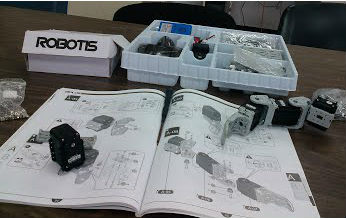
\includegraphics[scale=0.5]{imagenes/kitAfuera.jpg}
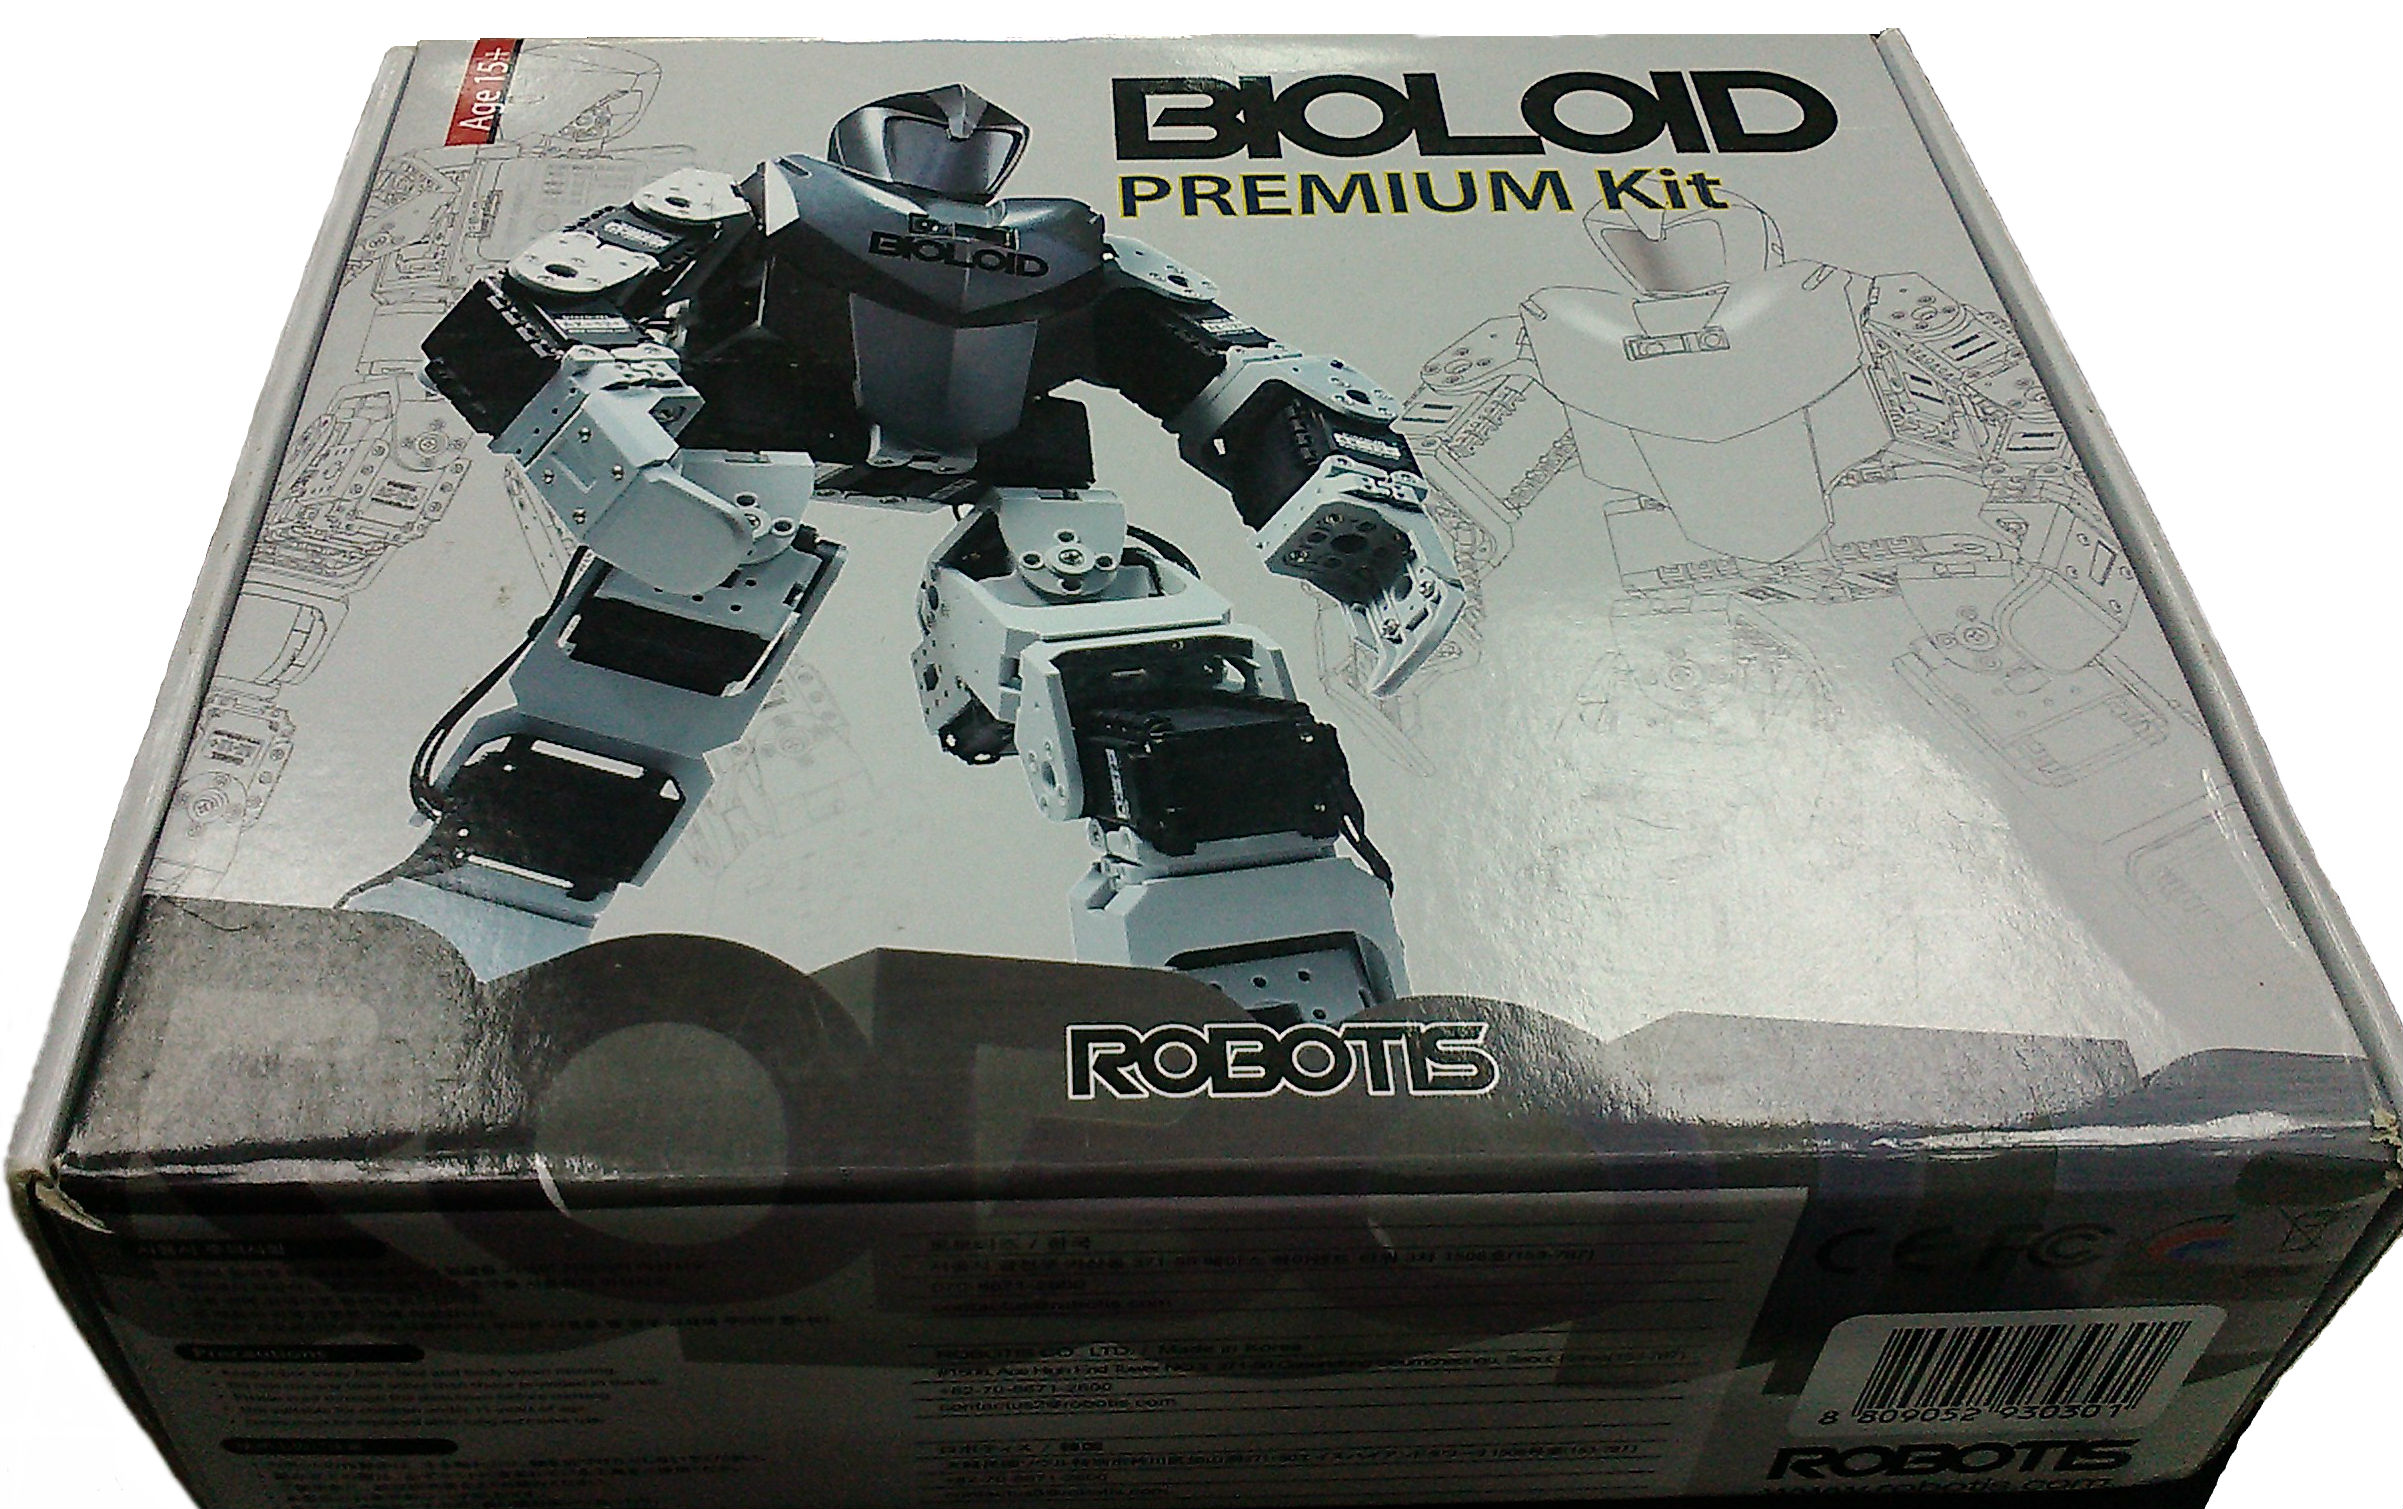
\includegraphics[scale=0.07]{imagenes/cajaKit.jpg}
\caption{Bioloid Premium Kit}
\label{fig:kit}
\end{figure}



\begin{itemize}

\item Motores Dynamixel Ax-12+: Son actuadores inteligentes y modulares que incorporan un reductor de engranajes, un motor DC de presión y un circuito de control con funcionalidad de red lo cual permite formar series o cadenas de motores (figura ~\ref{fig:motoresDc}), todo en un solo paquete \cite{manual}. 
\end{itemize}

\begin{figure}[hbtp]

\centering
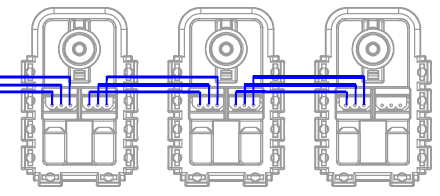
\includegraphics[scale=0.5]{imagenes/AX-12_serie.png}
\caption{Motores Dynamixel conectados en serie}
\label{fig:motoresDc}
\end{figure}

\begin{itemize}
\item Gyro: Es un giroscopio de la marca Robotis que mide la velocidad angular. Se encuentra diseñado para mantener el balance del robot y ser usado para otras aplicaciones de movimiento\cite{gyro}. En figura ~\ref{fig:gyro} se puede observar su estructura.  

\end{itemize}

\begin{figure}[hbtp]
\centering
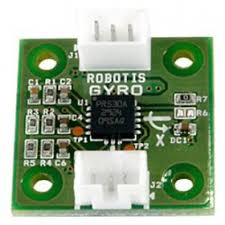
\includegraphics[scale=0.35]{imagenes/gyro.jpg}
\caption{Sensor Gyro}
\label{fig:gyro}
\end{figure}

\begin{itemize}
\item Arbotix: El controlador ArbotiX es una solución de control avanzado para manejar algunos tipos de servos Dynamixel y robots
basados en Bioloid. Incorpora un potente microcontrolador AVR, radio inalámbrica XBEE, conductores de motor dual, y cabeceras
de estilo servo de 3 pines para entrada/salida digital y analógica \cite{arbotix}.

\end{itemize}

%\begin{figure}[hbtp]
%\centering
%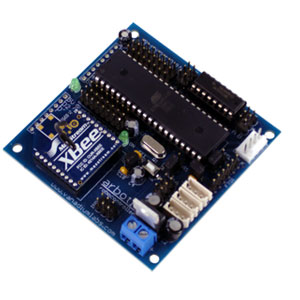
\includegraphics[scale=0.5]{imagenes/ARBOTIX.JPG}
%\caption{Tarjeta controladora ArbotiX}
%\end{figure}

\begin{itemize}
\item FTDI (Future Technology Devices International) : Es una tarjeta controladora  (figura ~\ref{fig:ftdi}) que ofrece el servicio de conversión de  datos de USB a UART. Permite la comunicación entre diferentes dispositivos \cite{ftdi}.

\end{itemize}

\begin{figure}[hbtp]
\centering
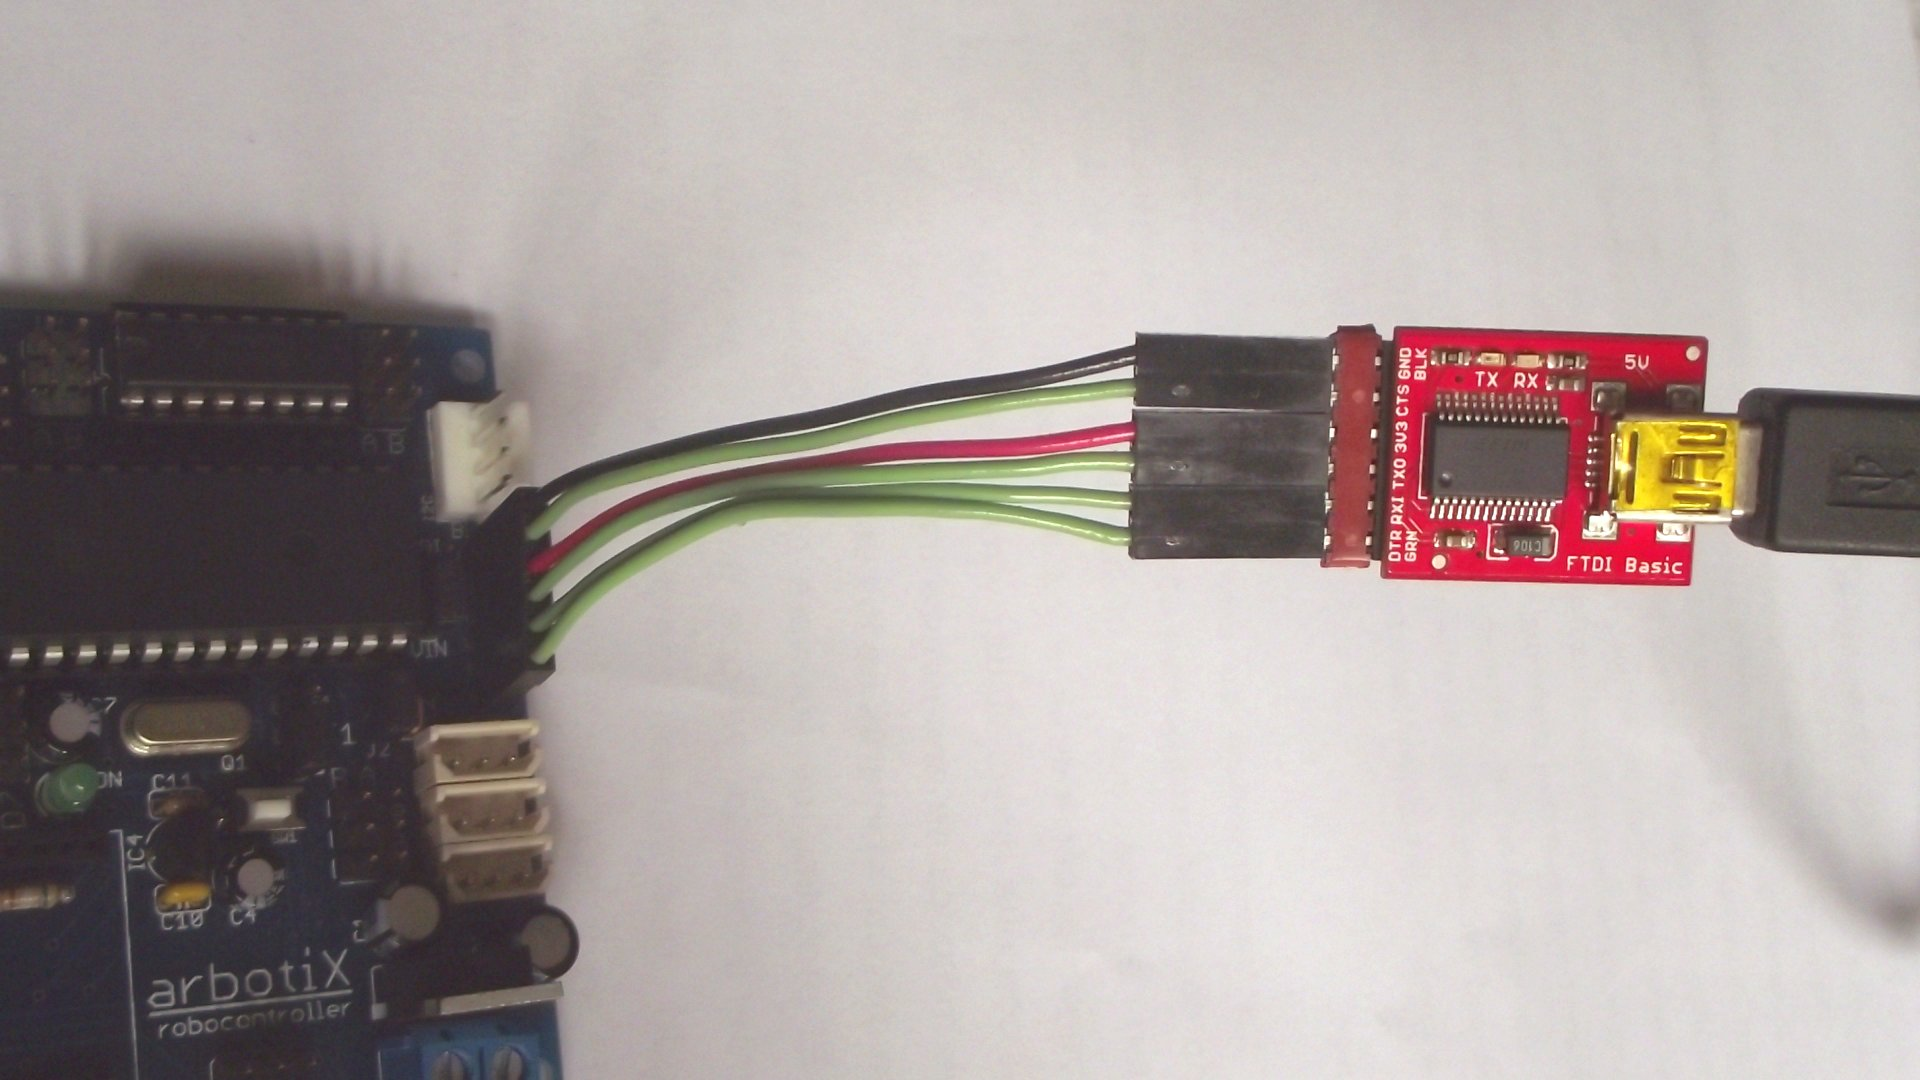
\includegraphics[scale=0.06]{imagenes/DSCF1162.jpg}
\caption{Chip FTDI conectado a la tarjeta Arbotix}
\label{fig:ftdi}
\end{figure}

\begin{itemize}
\item Extensor de puertos Bioloid : Permite aumentar el número de cadenas de servos conectados a la tarjeta (ver figura ~\ref{fig:ext}) \cite{hub}.
\end{itemize}

\begin{figure}[hbtp]
\centering
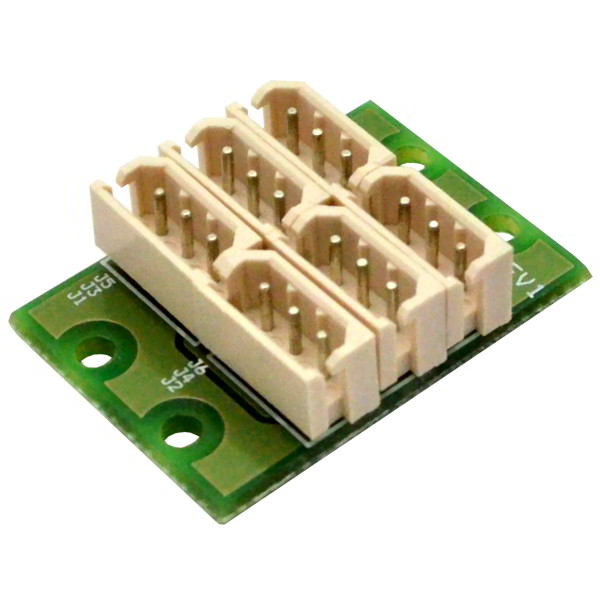
\includegraphics[scale=0.15]{imagenes/Dynamixel-AX-MX-6-Port-Extension-Hub-600x600.jpg}
\caption{Extensor de puertos Bioloid}
\label{fig:ext}
\end{figure}

\begin{itemize}
\item Micro servo motor anal\'ogico TG9e: Es un pequeño servomotor cuya capacidad de torque alcanza los 1.50 kg-cm \cite{microservo}. Permite ser controlado en posición en un rango de 180$^{\circ}$. Ver figura ~\ref{fig:Servo}.  

\end{itemize}

\begin{figure}[hbtp]
\centering
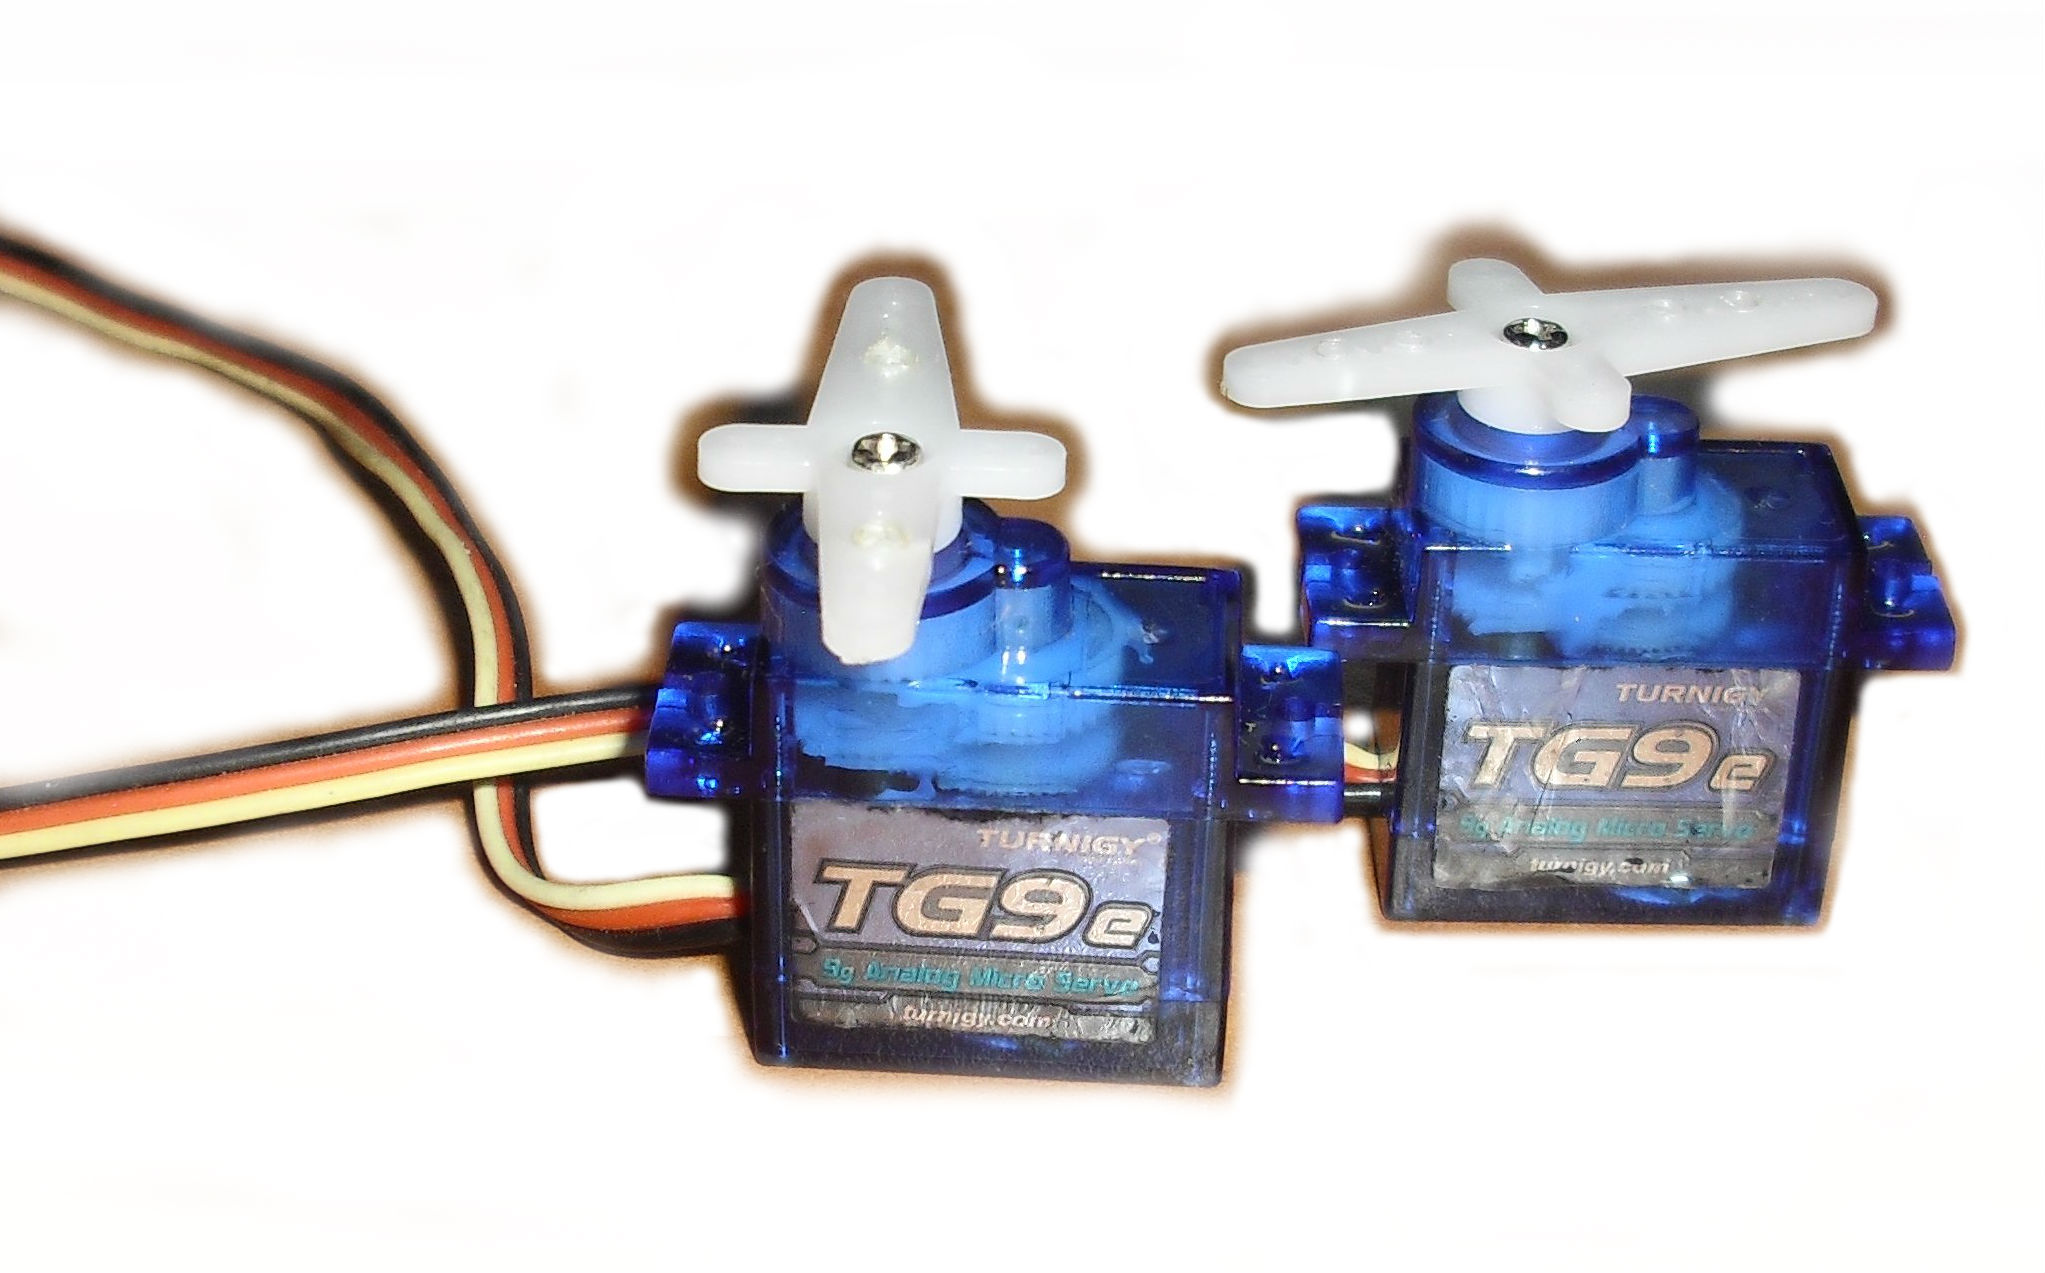
\includegraphics[scale=0.09]{imagenes/servosTg9B.jpg}

\caption{Micro Servomotores analógicos TG9e}

\label{fig:Servo}
\end{figure}

\begin{itemize}
\item Raspberry Pi: La Raspberry Pi es un ordenador del tamaño de una tarjeta de crédito a la que se puede conectar un televisor y un teclado. Se trata de un pequeño ordenador capaz de ser utilizado en proyectos de electrónica y para muchas de las tareas que una PC de escritorio hace, como hojas de cálculo, procesadores de texto y juegos \cite{raspberry}. Ver figura ~\ref{fig:Raspe}. La Raspberry Pi cuenta con un procesador gráfico que permite aligerar la carga del procesador central \cite{elLinux}. 

\end{itemize}

%imagen tomada de: %http://rayhightower.com/blog/2012/12/03/ruby-on-raspberry-pi/
\begin{figure}[hbtp]
\centering
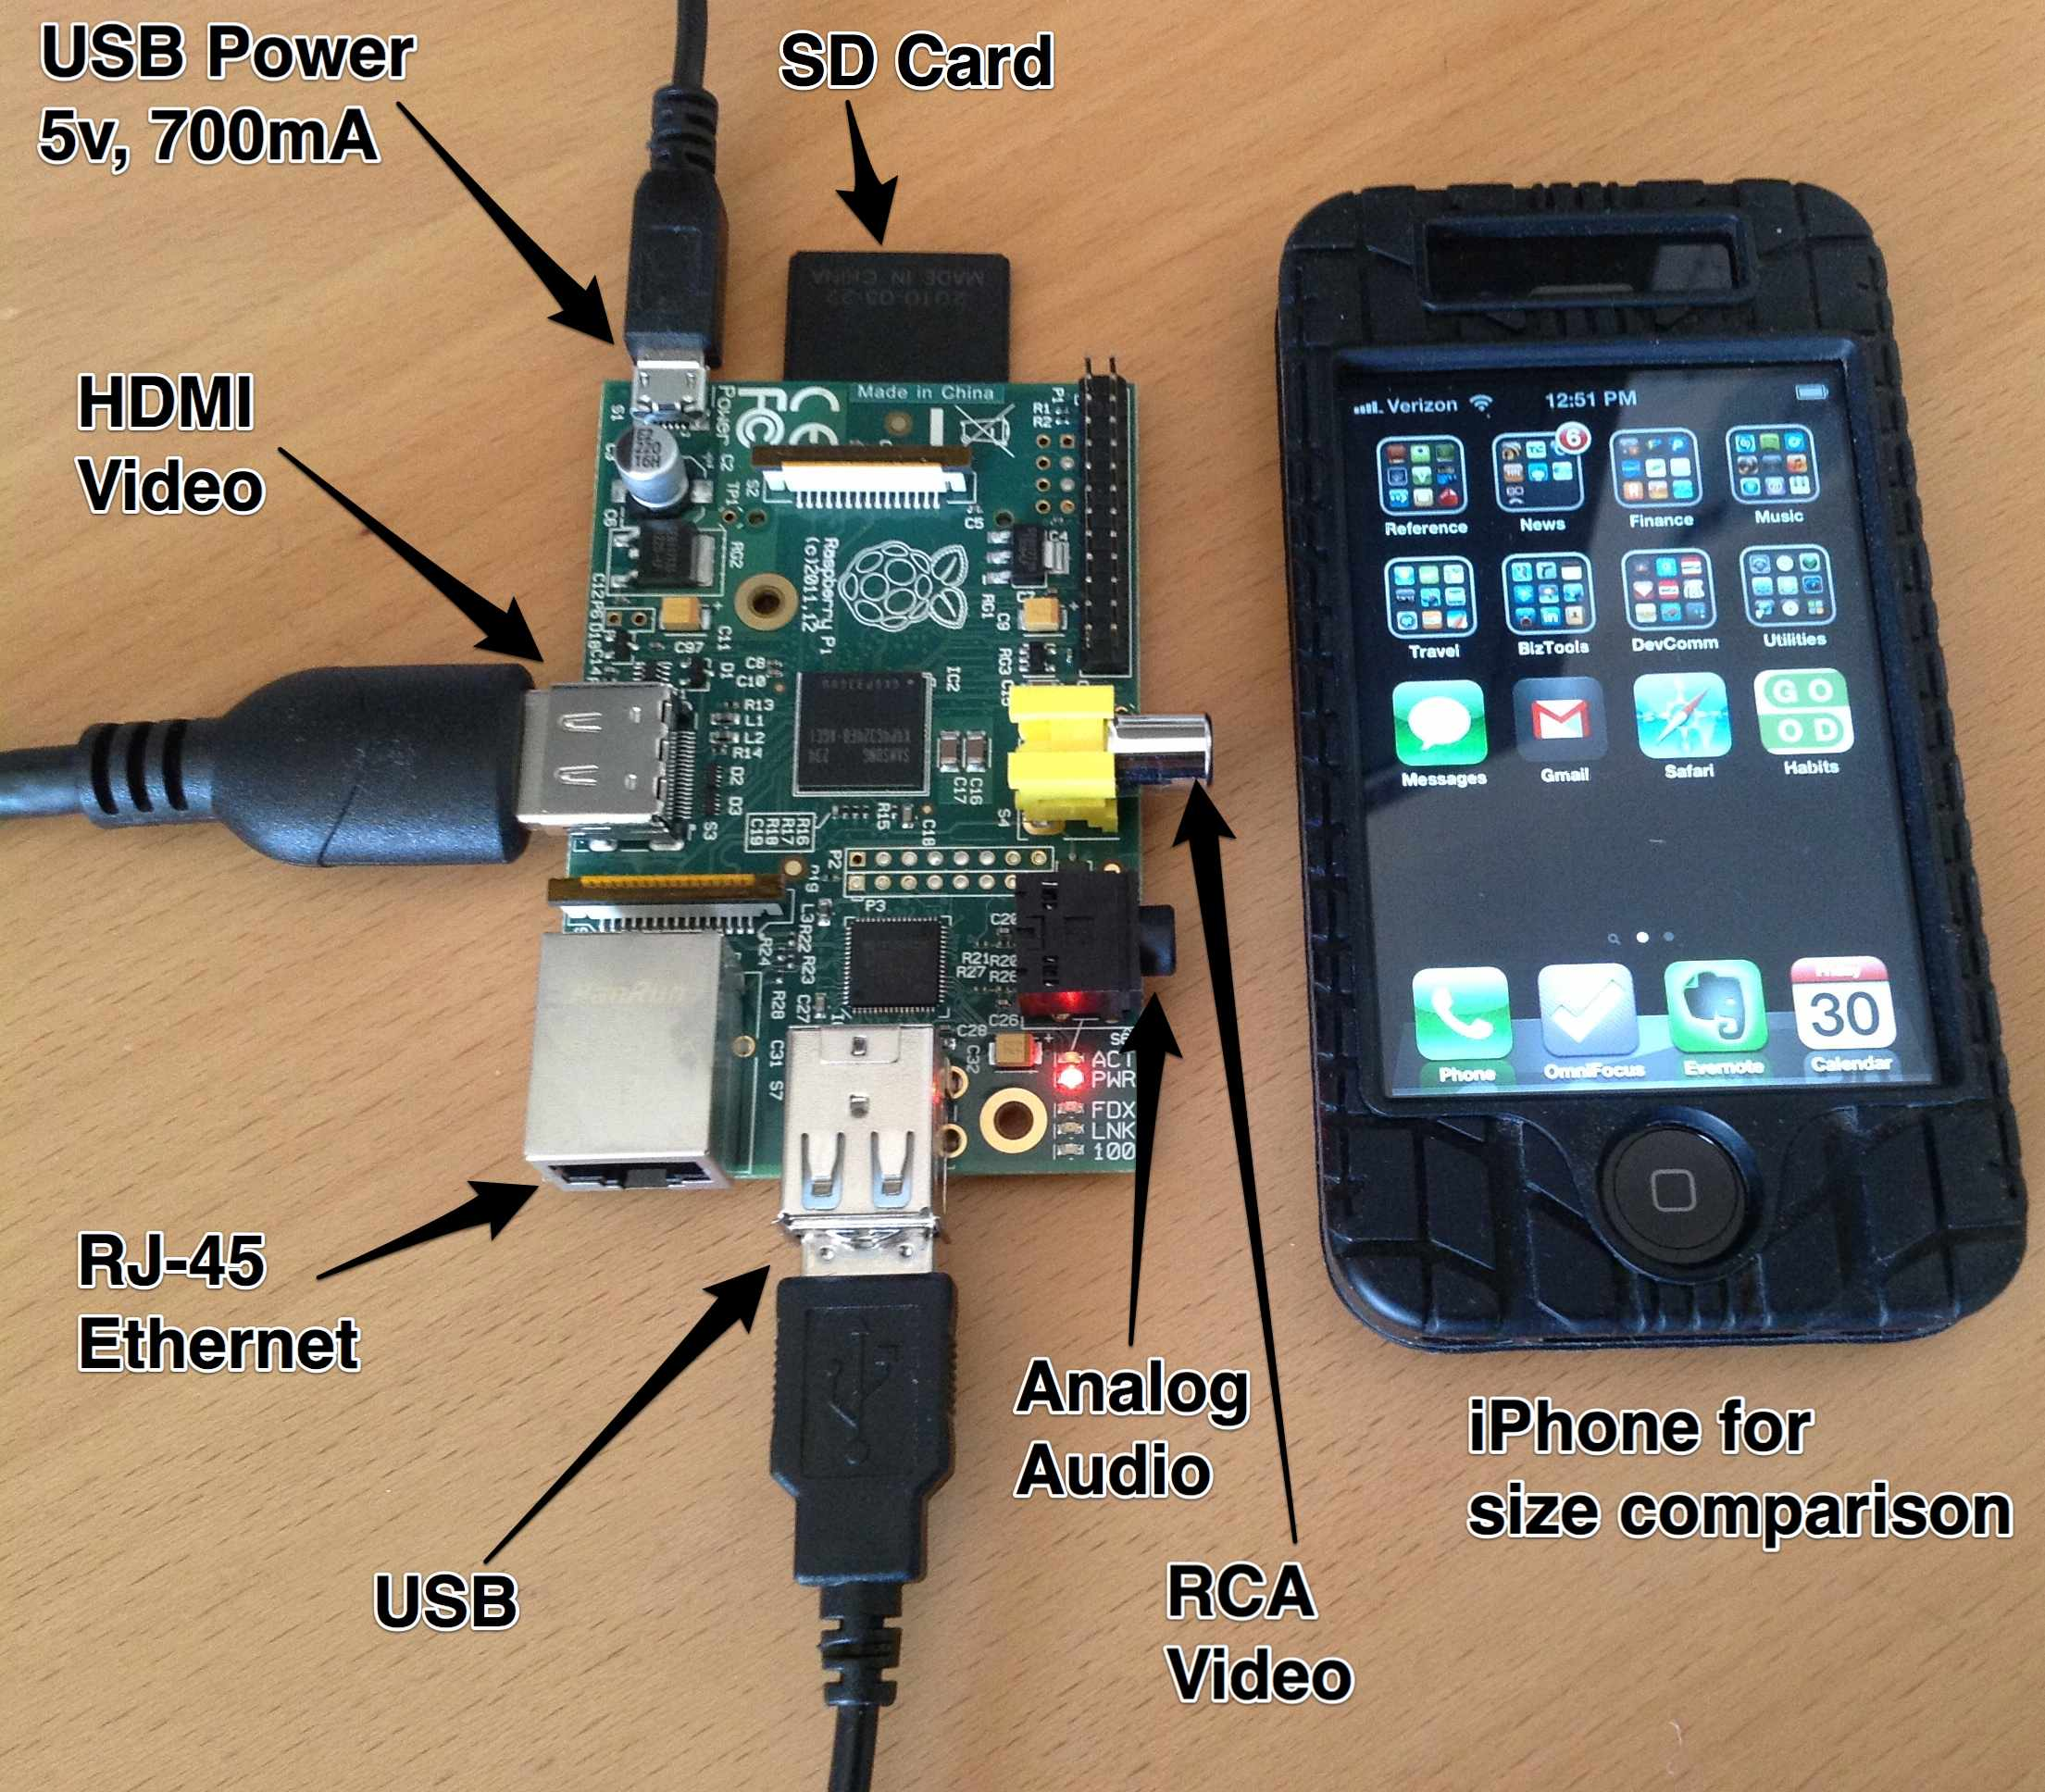
\includegraphics[scale=0.1]{imagenes/raspberry_pi_iphone.jpg}
\caption{Tarjeta Raspberry Pi con descripción de los puertos}
\label{fig:Raspe}
\end{figure}

\begin{itemize}
\item C\'amara Raspberry Pi: Es un sensor encargado de captar imagenes y grabar vídeos de alta definición. Se conecta a la Raspberry Pi con un cable de cinta plana de 15 cm en el puerto CSI. Tiene 5 megapíxeles de foco fijo que soporta los modos de vídeo de 1080x30, 720x60 y VGA90. Puede ser manejada con las librerías MMAL, V4L u otras librerías de terceros como la de Python \cite{raspberrycam}.(figura ~\ref{fig:came})  %(http://www.raspberrypi.org/products/camera-module/)

\end{itemize}

\begin{figure}[hbtp]
\centering
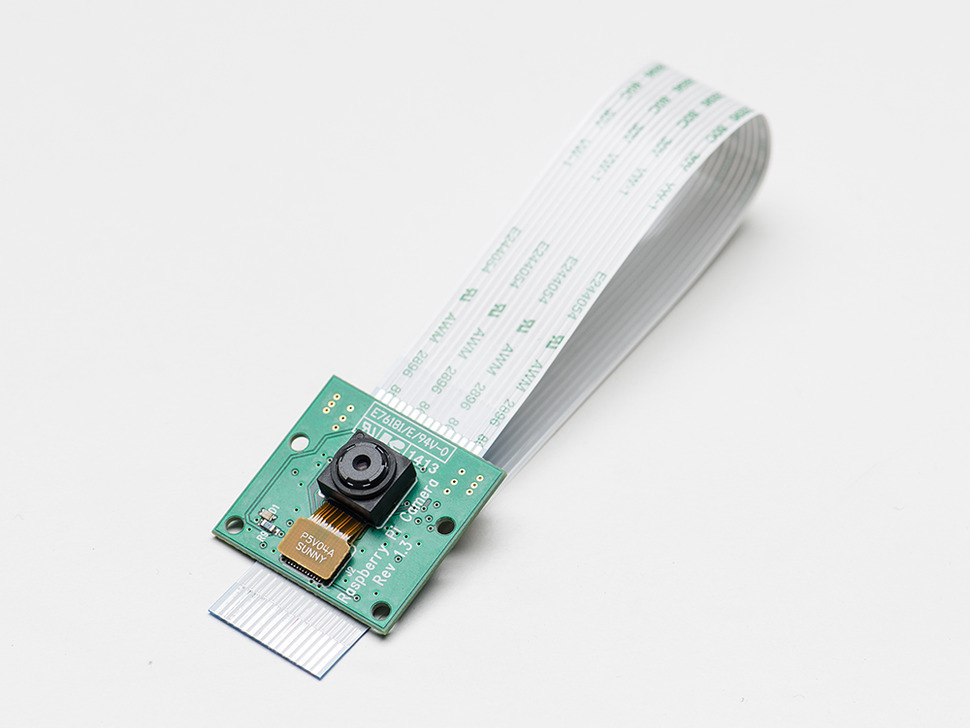
\includegraphics[scale=0.35]{imagenes/1367-01.jpg}
\caption{C\'amara Raspberry Pi}
\label{fig:came}
\end{figure}


\begin{itemize}
\item Batería de polímero de litio (Lipo): Es la fuente de poder usada para los motores y componentes electr\'onicos. La batería usada es de 11.1 voltios y 1 amperio. \cite{bateria}
\end{itemize}


\begin{figure}[hbtp]
\centering
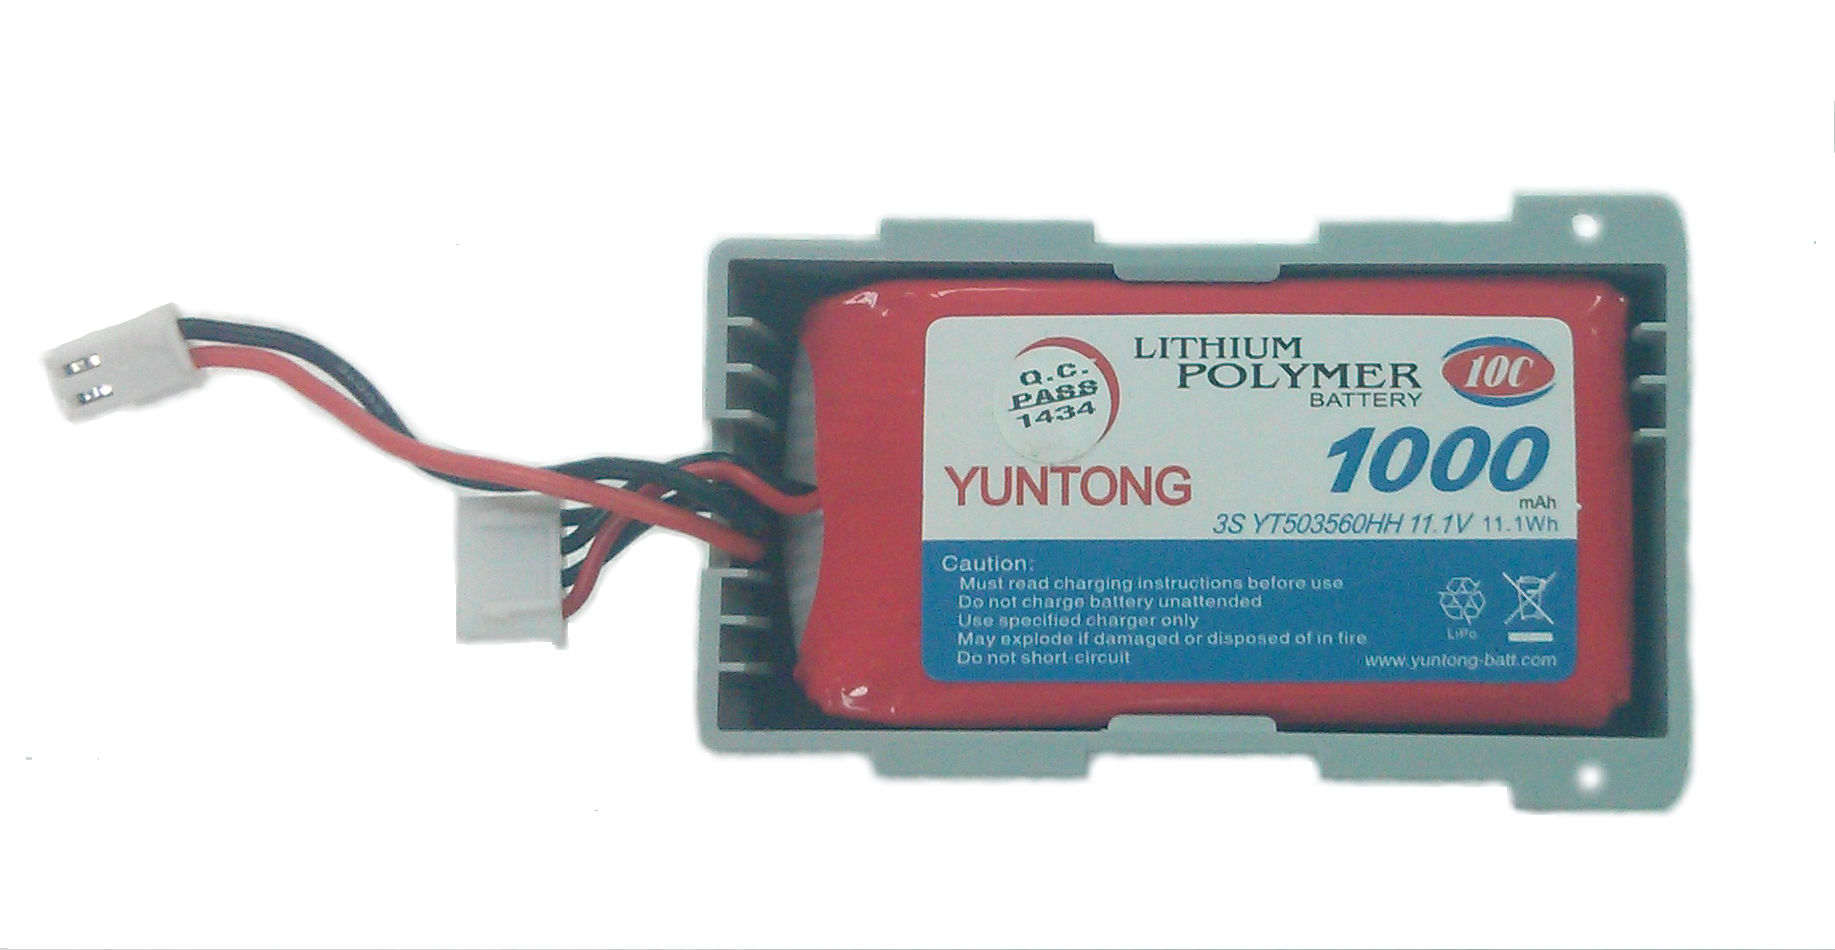
\includegraphics[scale=0.1]{imagenes/bateriaLipo.jpg}
\caption{Batería Lipo}
\label{bateria}
\end{figure}

\begin{itemize}
\item Circuito con regulador de 5v: Es un circuito diseñado y construido para este proyecto cuya finalidad es regular la entrada de la corriente. Por una de las salidas se expulsa 5v y por la otra se mantiene el mismo voltaje de entrada. 
\end{itemize}

%\begin{figure}[hbtp]
%\centering
%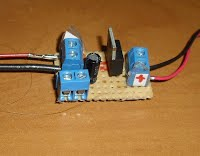
\includegraphics[scale=0.7]{imagenes/circuito.jpg}
%\caption{Lipo}
%\end{figure}

\label{subsection:construccion}
\subsection{Construcción}
Para la construcción del robot se utilizó el kit de piezas Bioloid Premium de marca Robotis el cual incluye motores Dynamixel Ax-12+, una tarjeta controladora CM-510, un sensor Gyro, un manual, entre otros elementos. El manual incluye las instrucciones de como armar varios modelos de humanoide, el utilizado en este proyecto es el tipo B, haciendo uso de 16 motores. En las figuras ~\ref{fig:frontal} y ~\ref{fig:trasera1} se puede observar la estructura del robot que aparece en el manual del kit. 

\begin{figure}[hbtp]
\centering
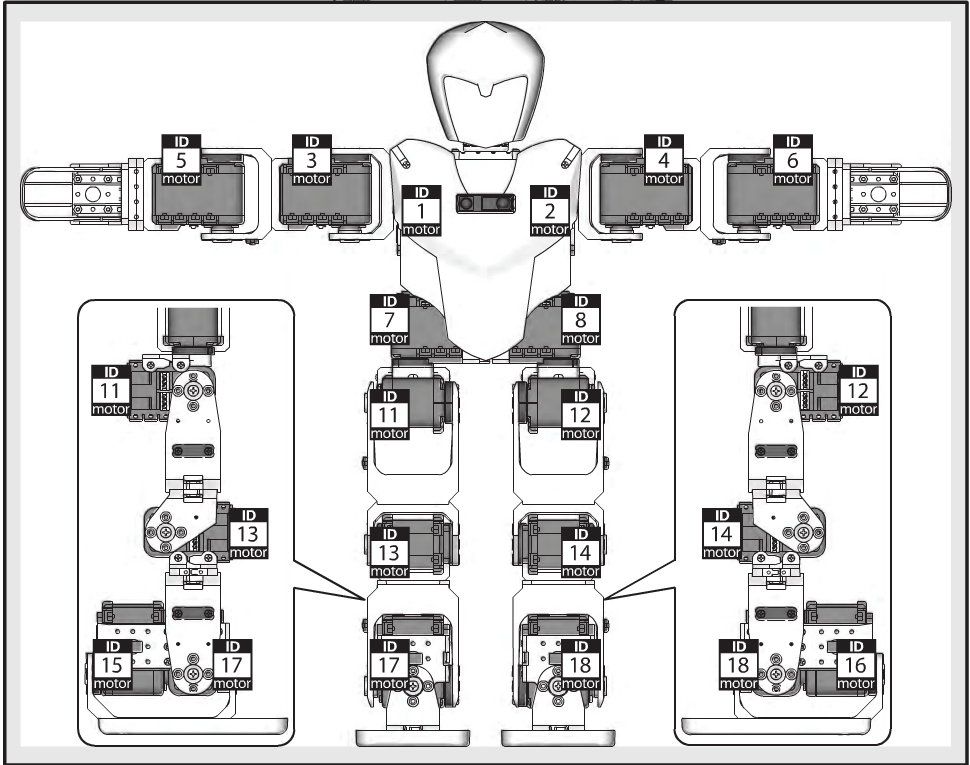
\includegraphics[scale=0.3]{imagenes/Robot.png}
\caption{Vista frontal del robot, tipo B, tomada del manual. Se puede apreciar la identificación ‘ID’ de cada motor Dynamixel Ax-12+. Nota: los motores 9 y 10 no se utilizan.}
\label{fig:frontal}
\end{figure}

\begin{figure}[hbtp]
\centering
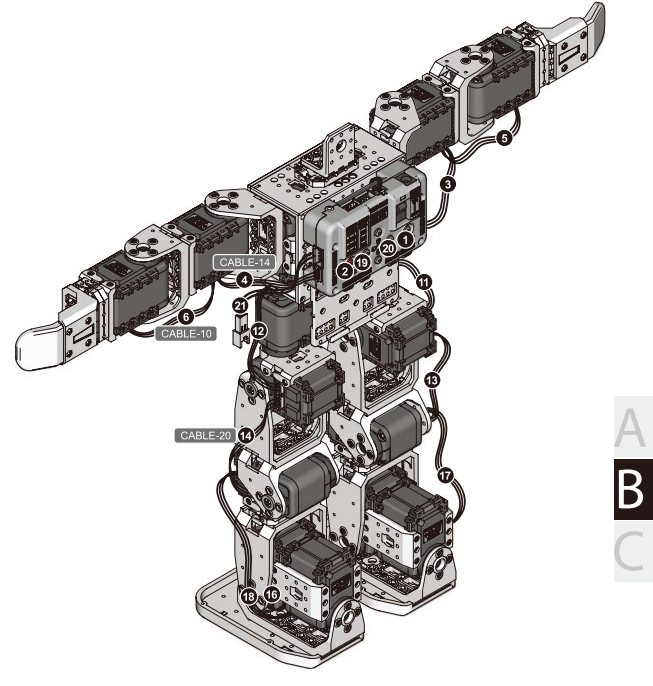
\includegraphics[scale=0.3]{imagenes/RobotTrasero.png}
\caption{Vista trasera del robot con la tarjeta CM-510, tomada del manual del kit Bioloid.}
\label{fig:trasera1}
\end{figure}


El kit bioloid incluye una tarjeta controladora CM-510 la cual fue sustituida por la tarjeta controladora de software libre Arbotix. La utilización de la tarjeta Arbotix permite una mayor flexibilidad en el control de motores y la incorporación de una variedad de sensores no soportados por la tarjeta CM-510.
Además, la tarjeta Arbotix posee mayor soporte y amplitud en la comunicación entre distintos dispositivos. 

En la figura ~\ref{fig:trasera2} se puede observar la estructura del robot con la Arbotix incorporada. En la parte interna del tronco del robot se sitúa el sensor Gyro.

\begin{figure}[hbtp]
\centering
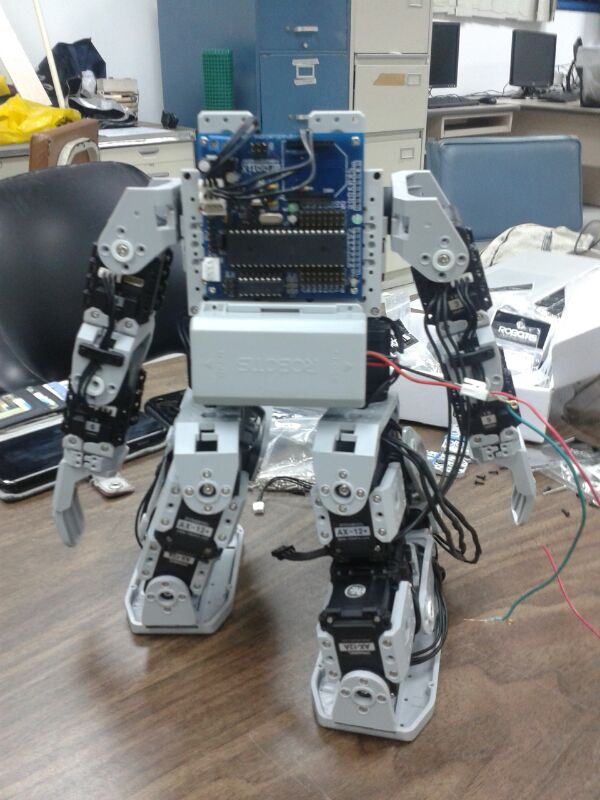
\includegraphics[scale=0.2]{imagenes/traseroDeJunny.jpg}
\caption{Vista trasera del robot con la Arbotix}
\label{fig:trasera2}
\end{figure}



Para el movimiento de la cámara se ha incorporado dos micro servomotores, uno para el movimiento horizontal y otro para el vertical. La conexión de uno de estos motores se ilustra en la figura ~\ref{fig:arbotixConectados}, en donde se puede observar que se encuentra conectado al puerto B de los denominados 'Hobby Servo ports'. La cámara ha sido conectada a la Raspberry Pi en el puerto CSI (ver la figura ~\ref{fig:camACSI}). El resultado de estas tres piezas instaladas en el robot se puede apreciar en la figura ~\ref{fig:servosycam}.

%\begin{figure}[hbtp]
%\centering
%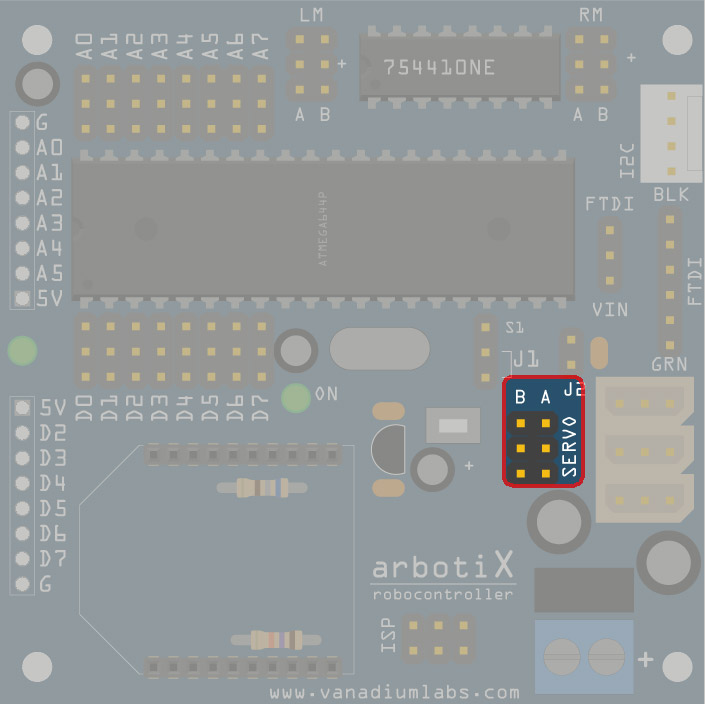
\includegraphics[scale=0.2]{imagenes/arbotix_hobby_servo.jpg}
%\caption{Ilustración de los puertos Hobby de la Arbotix}
%\label{fig:puertosHobby}
%\end{figure}

\begin{figure}[hbtp]
\centering
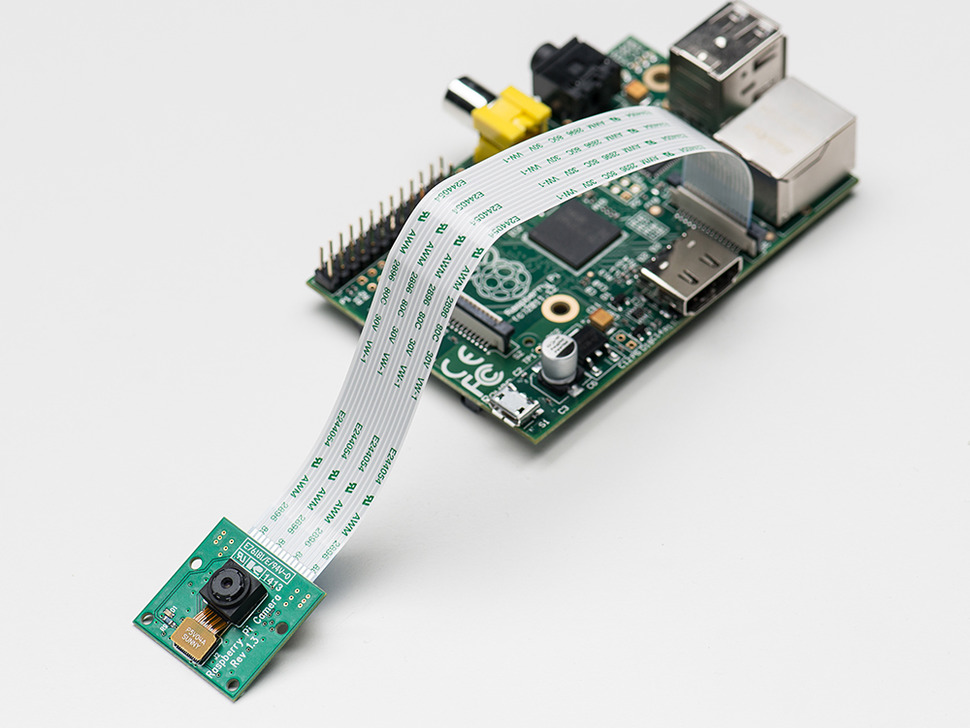
\includegraphics[scale=0.6]{imagenes/raspbCam.jpg}
\caption{C\'amara Raspberry Pi conectada al puerto CSI de la tarjeta}
\label{fig:camACSI}
\end{figure}
 
\begin{figure}[hbtp]
\centering
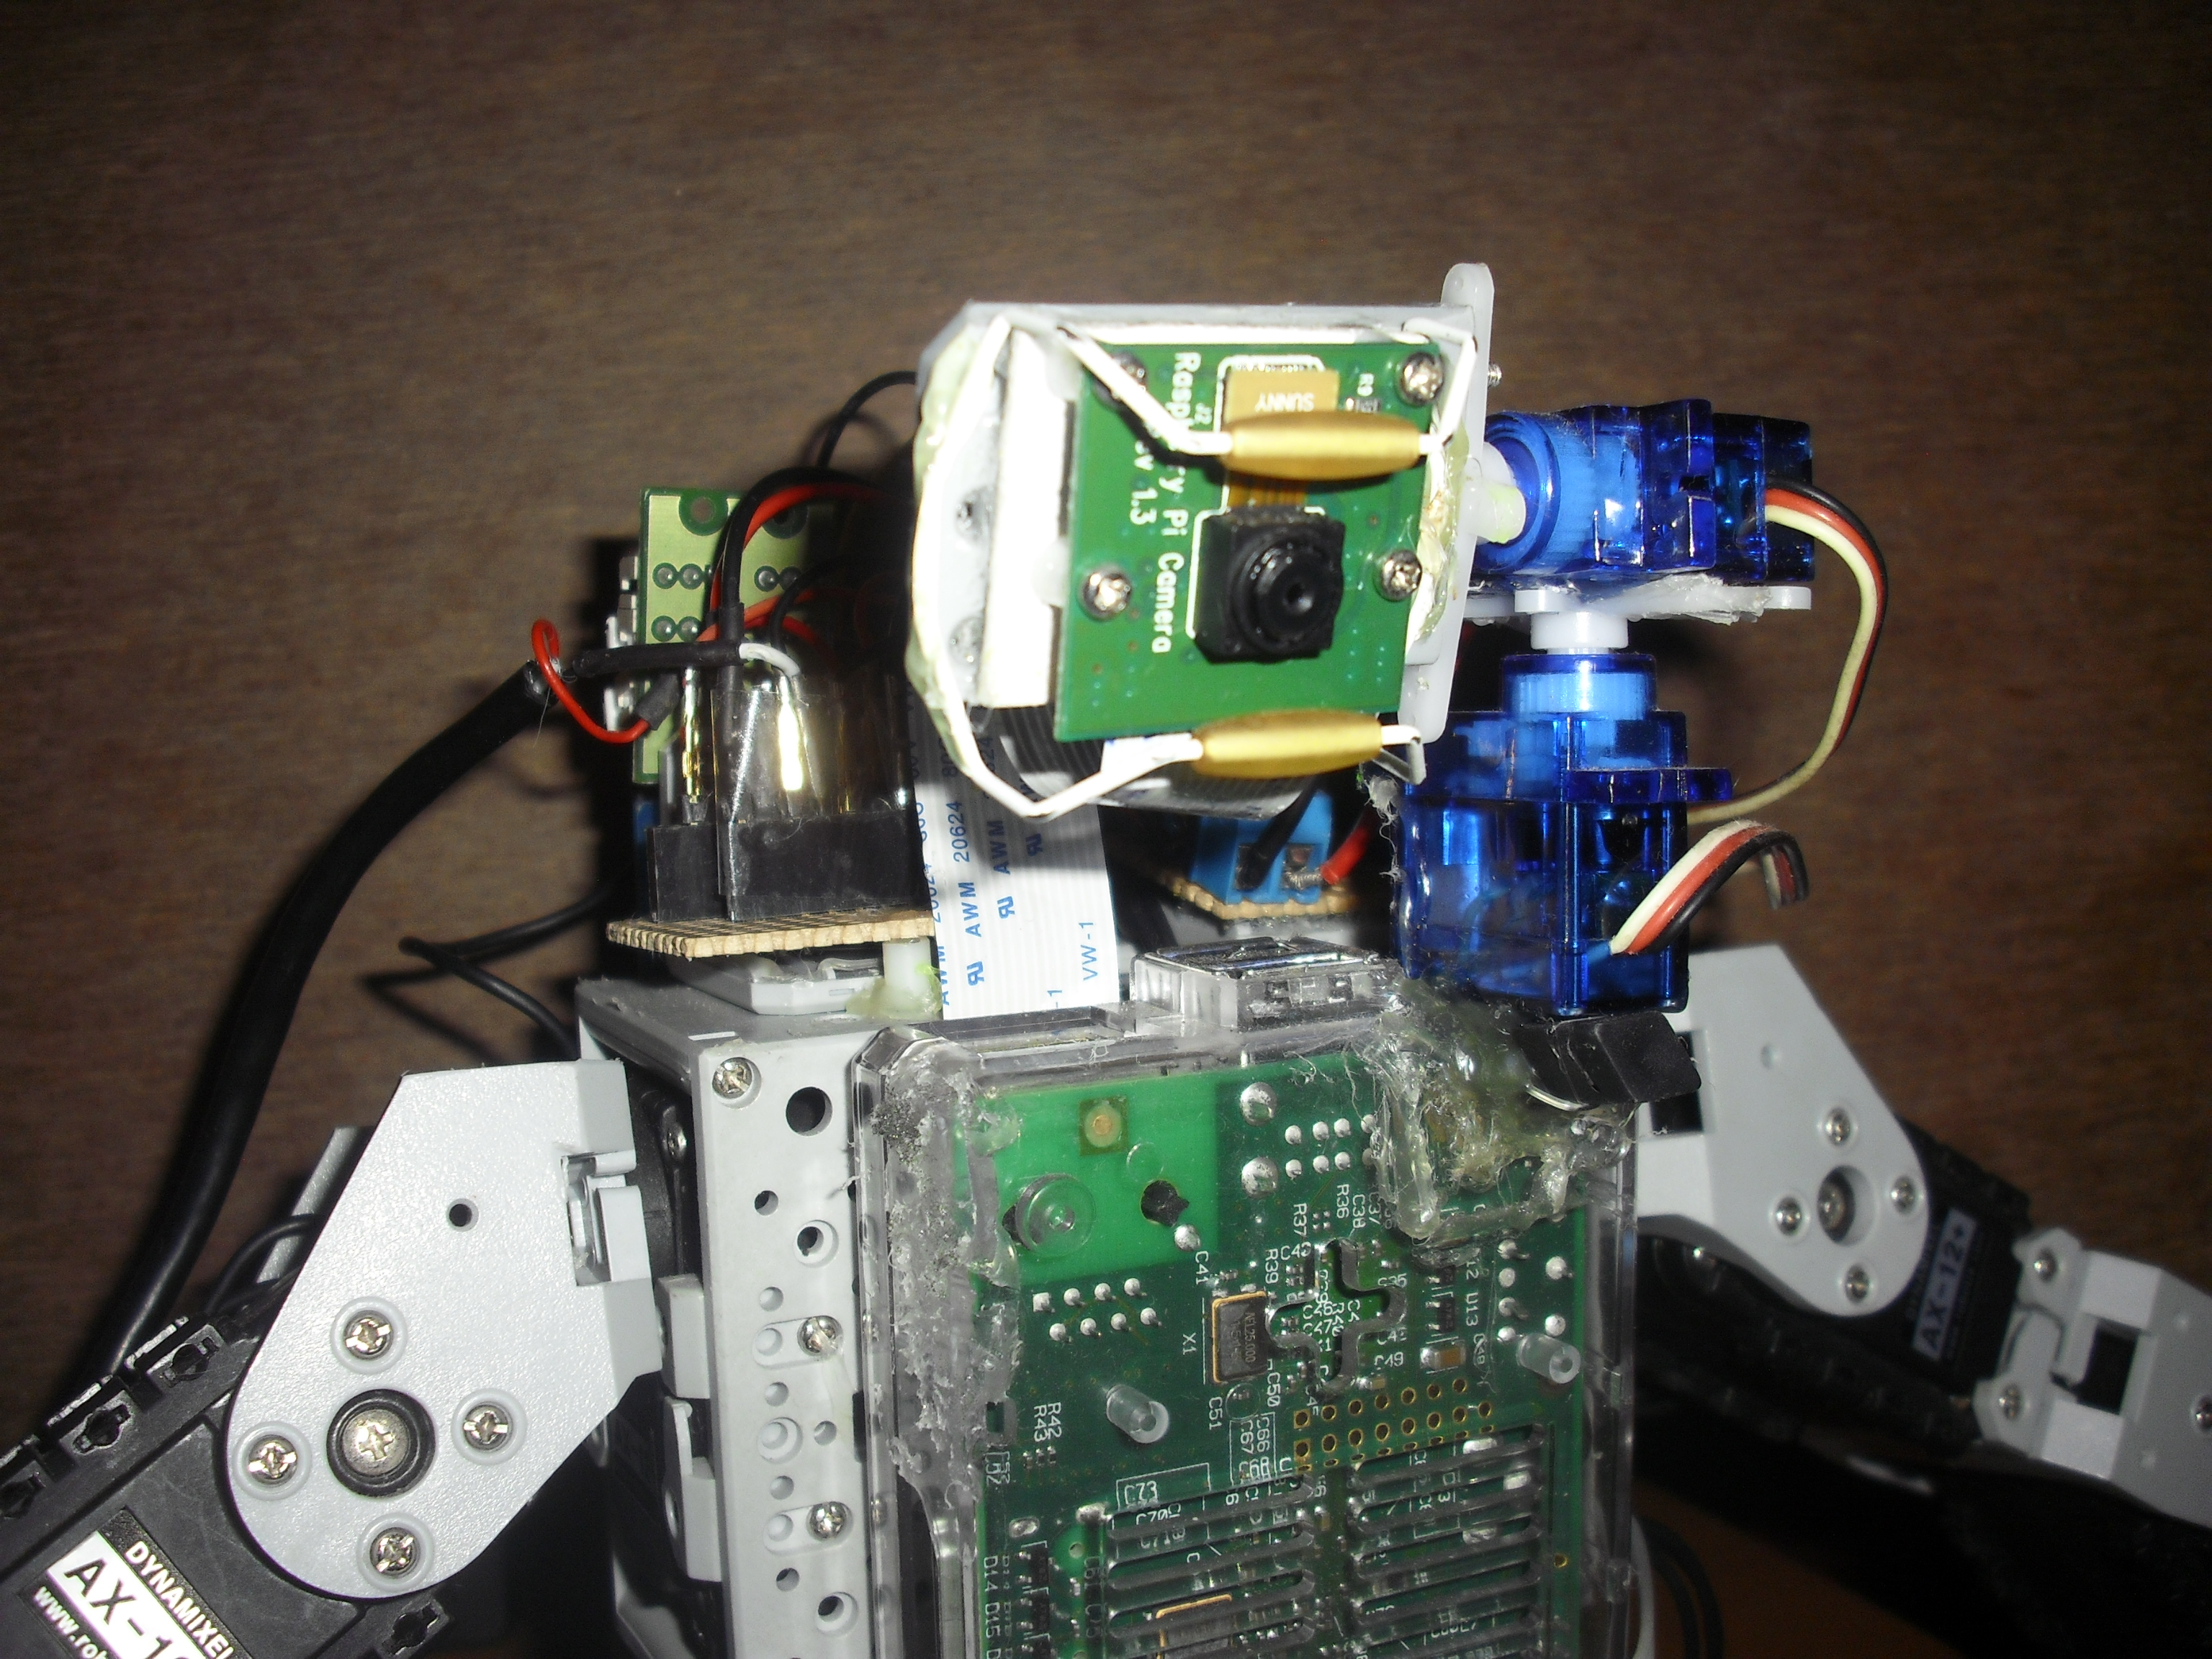
\includegraphics[scale=0.08]{imagenes/servosYcamara.JPG}
\caption{Vista delantera del robot con la cámara y servomotores instalados}
\label{fig:servosycam}
\end{figure}

Los motores Dynamixel se conectan a la controladora Arbotix por medio de los puertos Bioloid de la tarjeta. El diseño de Junny posee cuatro extremidades: dos brazos y dos piernas, por lo que naturalmente, el conjunto de motores, se puede descomponer en cuatro cadenas o series separadas. Sin embargo la Arbotix s\'olo cuenta con tres puertos Bioloid. Se consideró la opción de unir dos extremidades pero ello implicaba limitaciones en el movimiento del robot, por lo tanto se optó por agregar un expansor de puertos Bioloid y así conectar cada extremidad en un puerto diferente. La forma en la que se ha conectado estos motores se ejemplifica en la figura ~\ref{fig:arbotixConectados}. 

\begin{figure}[hbtp]
\centering
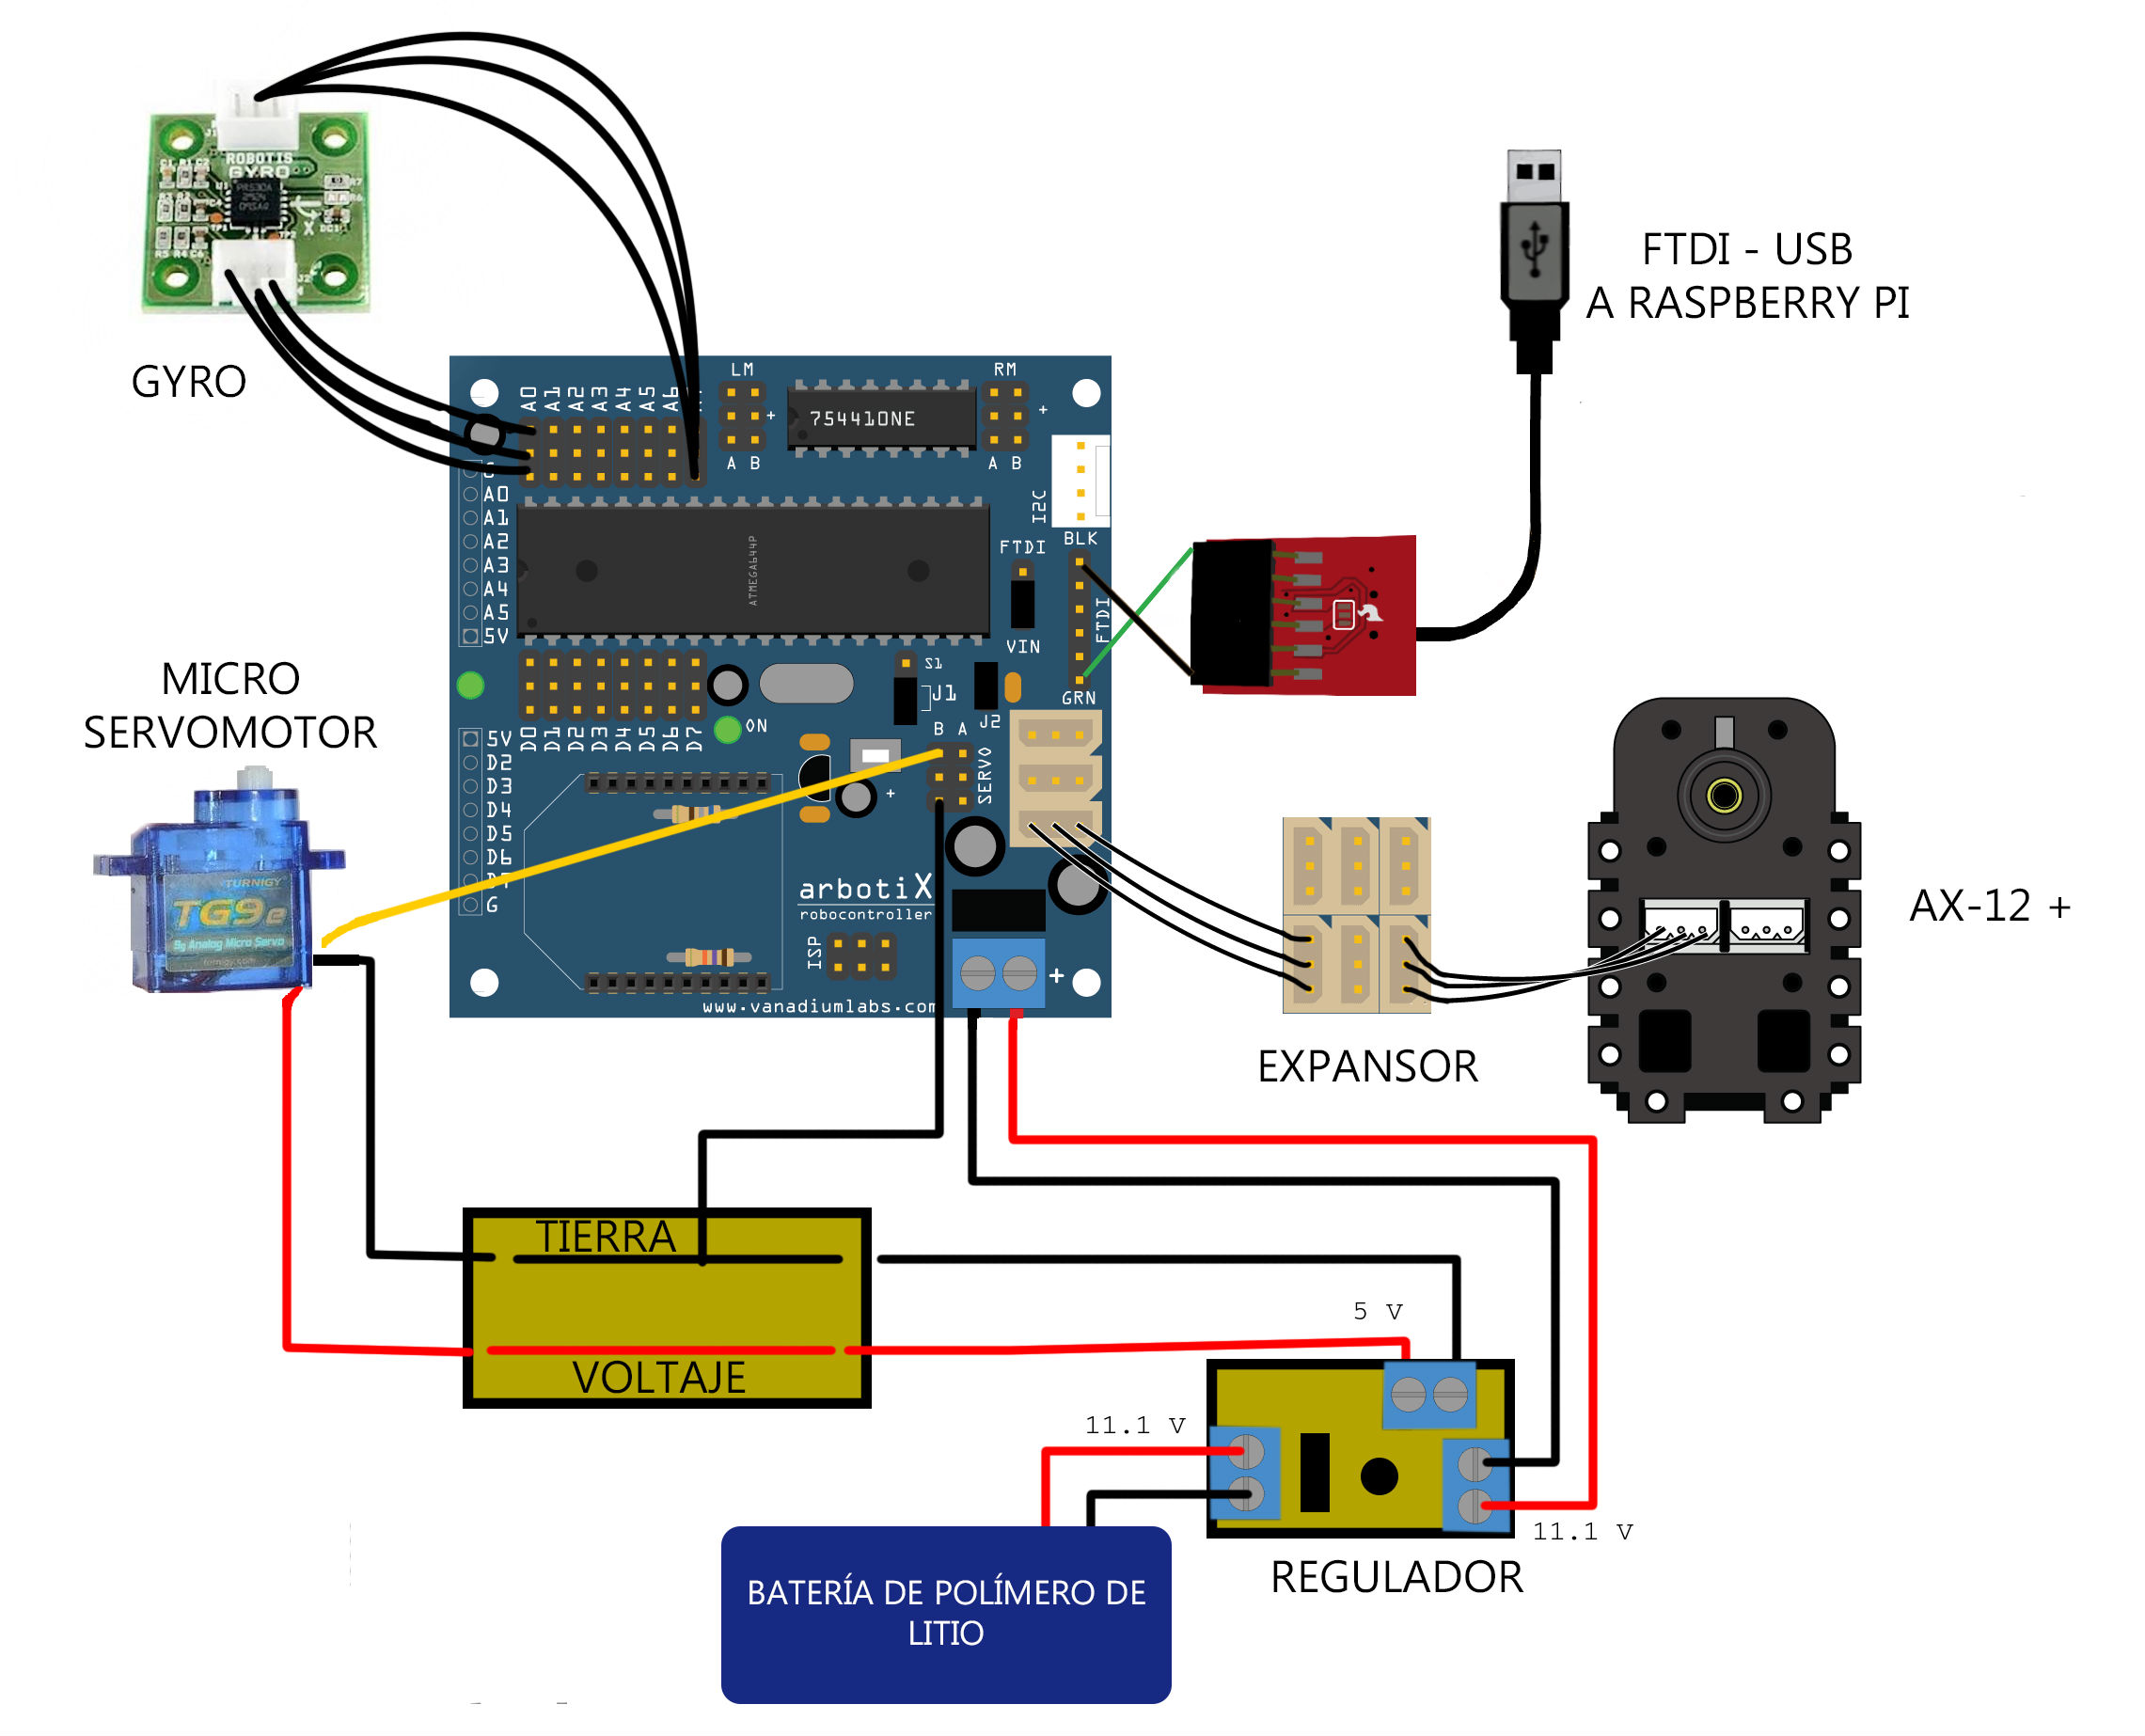
\includegraphics[scale=0.2]{imagenes/arbotix_componentes1.jpg}
\caption{Tarjeta controladora Arbotix y componentes conectados }
\label{fig:arbotixConectados}
\end{figure}

La comunicación de la tarjeta de Arbotix con la computadora, incluso con la Raspberry Pi, se realiza a través del puerto FTDI por medio un chip conectado como lo ilustra la figura ~\ref{fig:arbotixConectados}.

Como fuente de poder se utilizó una batería de polímero de litio de 11.1 V y 1 amp. Debido a que no todos los componentes poseen las mismas exigencias con respecto a voltaje y amperaje, se realizó un regulador (ver figura ~\ref{fig:circuito}) con una salida de 5 voltios para la tarjeta Raspberry Pi y dos micro servomotores, y otra salida de 11.1 V para la tarjeta Arbotix que a su vez alimenta a los componentes conectados en ella (motores Dynamixel y Giroscopio). Si bien la tarjeta Arbotix posee un regulador interno de cinco voltios la opción de conectar todo a la salida de 5 V del regulador no era posible, dado que los motores Dynamixel requieren alimentación de 11 voltios.

\begin{figure}[hbtp]
\centering
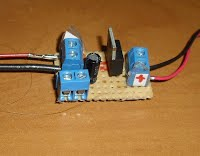
\includegraphics[scale=0.5]{imagenes/circuito.jpg}
\caption{Circuito con entrada de 11.1 V. Una salida de 5 V para los micro servomotores anal\'ogicos y tarjeta Raspberry Pi. Otra salida de 11.1 V para alimentar la controladora Arbotix.}
\label{fig:circuito}
\end{figure}

